\section{K-means Clustering}
\subsection{Theory}
The way that K-means clustering works is that there is a $C_1,...,C_k$ sets that contains part of the observations. These sets needs to satisfy two properties.
\begin{enumerate}
	\item $ C_1 \cup C_2 \cup ... \cup C_K = \{ 1,...,n \}$ Which means each observation belongs to at least one of the K clusters.
	\item $ C_k \cap C_{k'} = \emptyset $ for all $k \neq k'$ Which means the clusters are non-overlapping basically no observation belongs to more then one cluster.
\end{enumerate}

The goal of K-means clustering is to find good clusters with as small as possible within-cluster-variation. The Equation \ref{fo:k-meansMini}, tries to partition the observations into K clusters to achieve this.
\begin{align}\label{fo:k-meansMini}
\sum_{k=1}^{k} WCV(C_K)
\end{align}
To do this we need a distance metric. The one that is typically used is Euclidean distance, given by $d = \sqrt{ (x_2 - x_1)^2 - (y_2 - y_1)^2 } $. Which means the distance between two points is the length of the path connecting them or in other words the straight-line distance between two points in a plane. In Equation \ref{fo:EuclideanDistance1} $ |C_k| $ represent the number of observations in the \textit{k}'th cluster.
\begin{align}\label{fo:EuclideanDistance1}
WCV(C_K) = \dfrac{1}{|C_k|}  \sum_{i,i' \in C_k}   \sum_{j=1}^{p}(x_ij - x_{i'}j)^2
\end{align}
If we combine our two formulas given in \ref{fo:k-meansMini} and \ref{fo:EuclideanDistance2} we will get a optimization problem that defines K-means clustering. Were we try to minimize $ C_1,...,C_k $.
\begin{align}\label{fo:EuclideanDistance2}
\sum_{k=1}^{k} \dfrac{1}{|C_k|}  \sum_{i,i' \in C_k}   \sum_{j=1}^{p}(x_ij - x_i'j)^2
\end{align}

The K-Means Clustering Algorithm works like this
\begin{enumerate}
	\item The k centroids are placed at random.
	\item Assign each observation to the nearest of the k clusters.
	\item Move the centroids to the center of their clusters. The new position of each centroid is calculated as the average position of all the points in its cluster.
\end{enumerate}
We keep repeating steps 2 and 3 until the algorithm converges( centroid stop moving a lot at each iteration ).

\subsection{Results} %TODO rewrite (remove code etc.)
\subsubsection*{LAB 10.5.1}
Lab 10.5.1 is using the k-means clustering to group data. The lab begins by making a normal distribution put into a 25x2 matrix and in which there are two clusters in the data. Then changing the first 25 observations with a mean shift relative to the next 25 observations.

Then running the K-means clustering with K = 2 and 20 iterations. As it can be seen output of the algorithm is a set of labels assigning each observation to one of the k groups. The way that these groups are made is by creating a centroid for each group. The centroids are the middle of the cluster and they capture the points closest to them and adds them to the cluster. The plot of this can be seen in figure \ref{fig:kmeansclusteringk2_20Iteration} on the right.

Next we run the K-means clustering with K = 3 and 20 iterations. The plot of this can be seen in figure \ref{fig:kmeansclusteringk2_20Iteration} on the left.

\begin{figure}[H]
	\centering
	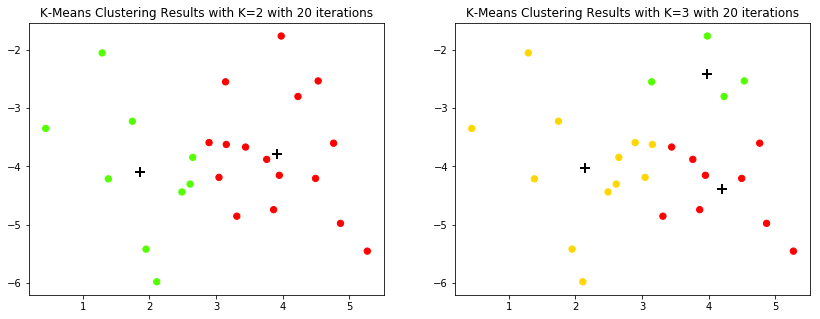
\includegraphics[width=0.7\textwidth]{clusteringMethods/kmeansclustering/fig/k-mean.png}
	\caption{K-Means Clustering Results with K=2 with 20 iterations on the right and  with K=3 with 20 iterations on the left}
	\label{fig:kmeansclusteringk2_20Iteration}
\end{figure}

While k-means clustering is a good algorithm, it is not without it's own flaws. When running K-means clustering with a large number of iterations, such as 20 since otherwise an undesirable local optimum may be obtained. Which simply means that, more than one run of the algorithm with randomized starting centroids could give a better result.


